
\section{Radiointerferometrie}
\sectionauthor{Benjamin Knöbel del Olmo, Ole Fleck, Aaron Gschwendt, Mara Germann}
\subsection{Kalibrierung der Radiointerferometriedaten}
Das Ziel dieses Projektteils ist es, Kalibrierungsfehler aus den Interferometriedaten herauszuprojizieren. Im Gegensatz zu Beobachtungen durch einzelne Antennenarrays wurde das Schwarze Loch M87* durch das Event-Horizon-Telescope (EHT) vermessen. Das EHT besteht aus Antennenstationen in verschiedensten Ländern (Chile, Spanien, Hawaii etc.). Der Abstand zwischen den Stationen ermöglicht es, sehr kleine Winkel aufzulösen (Ref Radiointerferometrie wg Formel!).
Bei der Messung treten vor allem zwei systematische Effekte vor: Dynamiken in der Atmosphäre führen zu Phasenverschiebungen und Temperaturschwankungen im Empfänger verursachen eine zeitabhängige Skalierung der Messdaten. Diese Störungen lassen sich durch die Formel
$$d_{abt\lambda}\rightarrow g_{at\lambda} \bar{g}_{bt\lambda}d_{abt\lambda}, \hspace{1cm} g_{at \lambda} \in \mathbb{C} \quad \forall a,t,\lambda $$
darstellen, wobei $a$ und $b$ für ein betrachtetes Antennenpaar (also Antenne $a$ und Antenne $b$) stehen und $g_{at\lambda}$,  $g_{bt\lambda}$ zwei für die jeweilige Antennenstörung beschreibende komplexe Zahlen sind: Der Abstandsbetrag spiegelt die Signalstärkenreduktion wider, während die komplexe Phase die Phasenverschiebung repräsentiert.
Um diese Effekte herauszukürzen, bestimmen wir die \emph{Closure Phases} und \emph{Closure Amplitudes}, eine bereinigte Form der gegebenen Daten. \emph{Closure Phases} behandeln die Phasenverschiebung der empfangenen Welle und \emph{Closure Amplitudes} die Änderung der Signalstärke. Für die Konstruktion der \emph{Closure Quantities} muss eine Funktion $f_{\lambda}$
\begin{equation}
d^0_{t\lambda}=f_{\lambda}(d_{ab\lambda},\quad \forall a,b)
\end{equation}
gefunden werden, die invariant ist unter
\begin{align}
d_{abt\lambda} &\rightarrow e^{i \phi_{at}} e^{-i\phi_{bt}} d_{abt\lambda}d(0)\\
d_{abt\lambda}&\rightarrow|g_{at\lambda}||g_{bt\lambda}|d_{abt\lambda}|
\end{align}
In der ersten Funktion werden die Verschiebungen in der Phase rausgekürzt, in der zweiten die Amplitudenverschiebung.
Für die \emph{Closure Phases} lautet eine geeignete Funktion
\begin{equation}f(d_{a,b},d_{b,c},d_{a,c})=d_{a,b}+d_{b,c}-d_{a,c}\end{equation}
Man kann zeigen, dass durch Einsetzen in die Funktion die Verschiebung der Daten herausgerechnet wird. 
Sei $\psi_n = e^{i \phi_{nt}}$ Dann gilt:
\begin{align}
f(\psi_a\bar{\psi_b} d_{a,b},\psi_b\bar{\psi_c}d_{b,c},\psi_a \bar{\psi_c} d_{a,c})&=\psi_1\bar{\psi_b}d_{a,b}+\psi_b\bar{\psi_c}d_{b,c}-\psi_a \bar{\psi_c} d_{a,c}\\
&=e^{i \phi_{a,t}-i\phi_{b,t}}d_{a,b}+e^{i \phi_{b,t}-i\phi_{c,t}}d_{b,c}-e^{i \phi_{a,t}-i\phi_{c,t}}d_{a,c}\\
&=d_{a,b}+d_{b,c}-d_{a,c}\\
&=f(d_{a,b},d_{b,c},d_{a,c}).
\end{align}
Für die \emph{Closure Amplitudes} lauten zwei mögliche Funktion:
\begin{align}
f(d_{a, b},d_{a, c},d_{a, d},d_{b, c},d_{b, d},d_{c, d})\overset{!}{=}\frac{d_{a,b}\cdot d_{c,d}}{d_{a,c} \cdot d_{b,d}}
\hspace{3mm}\text \quad {bzw.} \quad \hspace{3mm} \frac{d_{a,d}\cdot d_{b,c}}{d_{a,c} \cdot d_{b,d}}
\end{align}
Folgend werden die \emph{Closure Phases} für die verschiedenen Dreiergruppen bzw. die \emph{Closure Amplitudes} für die Vierergruppen aus Antennenpaaren berechnet. Da jedoch nicht alle Möglichkeiten unabhängig voneinander sind, müssen Redundanzen herausgerechnet werden.
Dafür wird eine Matrix erstellt, in der die Spalten alle möglichen Antennenpaare darstellen und die Zeilen alle linear unabhängige Möglichkeiten, die Antennenpaare zu verknüpfen, darstellt. Bei den  \emph{Closure Phases} stehen die Zahlen in der Matrix für das Vorzeichen, bei den \emph{Closure Amplitudes} für das Vorzeichen des Exponents. Folglich bedeuten Nullen, dass die Antennenpaare nicht verwendet werden.  Bei $n$ Antennen gibt es $\binom{n-1}{2}= \frac{1}{2}(n-1)(n-2)$ linear unabhängige Zeilen in der Matrix. 
Daher hat die $n=4$ \emph{Closure-Phase}-Matrix $\binom{4-1}{2}=3$ Zeilen:
\begin{equation}
\bordermatrix{
~ &(0,1)&(0,2)&(0,3)&(1,2)&(1,3)&(2,3)\cr
~&1&-1&0&1&0&0 \cr
~&1&0&-1&0&1&0 \cr
~&0&1&-1&0&0&1 \cr}
\end{equation}

Die \emph{Closure-Amplitude}-Matrix von $n$ Antennen hat $\frac{1}{2}n(n-3)$ linear unabhängige Reihen. Die $n=4$ \emph{Closure-Amplitude}-Matrix sieht folgendermaßen aus:
\begin{equation}
\bordermatrix{
~ &(0,1)&(0,2)&(0,3)&(1,2)&(1,3)&(2,3)\cr
~&1&-1&0&0&-1&1 \cr
~&0&-1&1&1&-1&0 \cr
}
\end{equation}
Um die \emph{Closure Phase} Matrizen zu generieren, verwenden wir folgende Funktion. 
\begin{verbatim}
def genPhaseMatrix(n):
    O=math.comb(n,2)
    mat=np.empty(O,dtype=int)
    pos=[(x,y) for x in range(n) for y in range(x+1,n)]
    maxRank=math.comb(n-1,2)
    for i in range(0,n):
        for j in range(i+1,n):
            for k in range(j+1,n):
                row=np.zeros(O,dtype=int)
                row[pos.index((i,j)),]=1
                row[pos.index((i,k))]=-1
                row[pos.index((j,k))]=1
                newMat=np.vstack([mat,row])
                rnk= np.linalg.matrix_rank(newMat)
                if rnk>np.linalg.matrix_rank(mat):
                    mat=newMat
                    if rnk==maxRank:
                        return mat[1:,:]
\end{verbatim}
Die Funktion nimmt als Parameter die Anzahl an Antennen. Zunächst erstellt sie ein leeres Numpy-Array mit einer Zeile für jedes mögliches Antennenpaar. In dem Array wird die Matrix zeilenweise erzeugt. Dann werden alle mögliche Kombinationen von drei Antennen durchlaufen. Ist die Kombination linear unabhängig zu der bereits bestehende Matrix, wird sie der Matrix zugefügt. Dies wird so oft wiederholt, bis entweder alle Möglichkeiten durchgegangen oder die maximale Zeilenanzahl der Matrix erreicht wird. \emph{Amplitude-Phase}-Matrizen werden analog generiert.

Nachdem die \emph{Closure Quantities} erstellt wurden, werden die Daten der Antennen für jedes Zeitintervall in Phase und Amplitude getrennt und mit den \emph{Closure Quantities} Matrizen multipliziert. Da nicht zu jedem Zeitpunkt gleich viele Antennen aktiv sind, (z.B. weil sie im Schatten der Erde liegen) brauchen wir alle \emph{Closure}-Matrizen bis $n=7$ gilt.

Um schließlich ein Bild zu erzeugen, benötigen wir den Posterior aus dem Theorem von Bayes. Um diesen zu berechnen, setzen wir ein: 


\begin{equation}
P(\xi|d)= \frac {P(d|\xi)\cdot P(\xi)}{ P(d) }
\end{equation}

\begin{equation}
P(d|\xi)=  {P(d_{ph}|\xi)\cdot P(d_{amp}|\xi)}    
\end{equation}

Die Likelihood (1.12) besteht aus zwei Teilen: $P(d_{ph}|\xi)$, der Wahrscheinlichkeit der \emph{Closure Phases} gegeben die Parameter $\xi$ und $P(d_{am}| \xi)$, der Wahrscheinlichkeit der \emph{Closure Amplitudes} gegeben $\xi$ : 

Der negative Logarithmus des Posteriors
\begin{align} \label{k4.2.Posterior}
 -\log {P(\xi|d)} &= 
 \mathcal{H} (\xi|d) = \mathcal{H} (d_{ph}|\xi)+\mathcal{H} (d_{amp}|\xi)+\mathcal{H} (\xi) \\
&= \frac {1}{2}\cdot \Bigg[d_{ph} - f_{ph}(R(sky(\xi))) \Bigg]^\dagger N^{-1}_{ph} \Bigg[d_{ph} - f_{ph}(R(sky(\xi))) \Bigg] 
\\  & + \frac {1}{2}\cdot \Bigg[d_{amp} - f_{amp}(R(sky(\xi))) \Bigg]^\dagger N_{amp}^{-1}\Bigg[d_{ph} - f_{ph}(R(sky(\xi))) \Bigg] \nonumber
\\ & +  \frac {1}{2} \cdot \xi^\dagger \xi \nonumber  
\end{align} 
 erlaubt uns, Metric Gaussian Variational Inference, kurz MGVI \parencite{k4.2.mgvi} anzuwenden. Dabei wird der Parameter $\xi$ so optimiert, dass man mit einer durch $\xi$ definierten Normalverteilung eine möglichst kleine Differenz zum wahren Posterior erreicht \cref{k4.2.hiera}
Dadurch erhält man folgendes Bild:

\begin{figure}
    \centering
    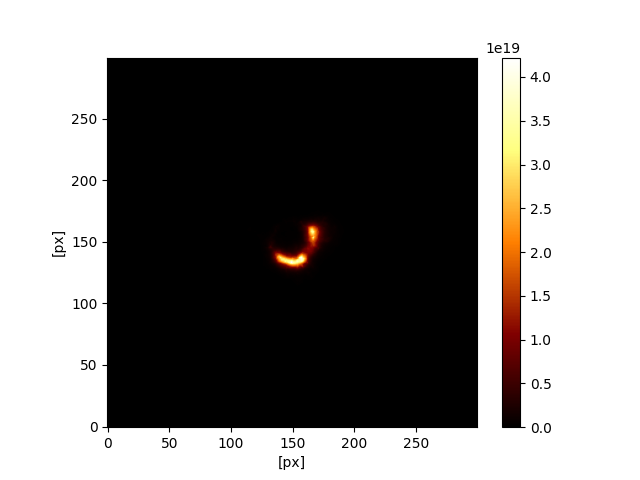
\includegraphics[width = 0.9\textwidth]{k4.2/black-hole-lin.png}
    \caption{Bild des Schwarzen Lochs M87*}
    \label{k4.2.black-hole-lin}
\end{figure}





\subsection{Radiointerferometrie-Response und Event-Horizon-Telescope-Daten}

Zur Rekonstruktion eines Bildes des Schwarzen Lochs M87* muss basierend auf den Daten des Event-Horizon-Telescopes zunächst eine Response-Funktion implementiert werden, um die Informationen vom Signal- in den Datenraum zu transferieren $s \mapsto d$. Mit der entsprechenden Implementierung wird sich der nachfolgende Abschnitt befassen.

Es werden Daten in Form von acht csv-Dateien verwendet, die im April 2017 aufgenommen wurden. Diese stammen von mehreren Messreihen und wurden zur weiteren Verarbeitung in Form von csv-Dateien gespeichert.
Um mit den Messwerten in Python arbeiten zu können, werden die csv-Dateien in NumPy-Arrays konvertiert. Durch das NumPy-Array werden die Daten aus den csv-Dateien auf einem zweidimensionalen Gitter abgebildet.

Zunächst müssen die Frequenzen der Radiowellen ausgelesen werden. Diese elektromagnetischen Wellen werden in unmittelbarer Nähe des Schwarzen Lochs ausgesandt. Es wurden die beiden Frequenzen $f_1 = 227,0707$ GHz und $f_2 = 229,0707$ GHz betrachtet. Darüber hinaus werden auch die Verbindungsvektoren zwischen den Antennen $uvw$ ausgelesen.

Um aus den Messwerten ein Bild erstellen zu können, wird die Anzahl der Pixel sowohl in x-, als auch in y-Richtung auf zunächst $100$ festgelegt, wobei dieser Wert variabel ist. Die Größe der Pixel ergibt sich für $\delta \theta$:
\[ \delta \theta = 1.22 \cdot \displaystyle\frac{\lambda}{D} = 1.22 \cdot \displaystyle\frac{c}{f \cdot D} \]

Da es sich bei dem Event Horizon Telescope um einen Zusammenschluss von Antennen auf der ganzen Welt handelt, ergibt sich ein Durchmesser von $D_{EHT} \approx D_{Erde} \approx 10.000km$. Desweiteren beschreibt $\lambda$ die Wellenlänge der Radiowellen und $c$ deren Ausbreitungsgeschwindigkeit, die der Lichtgeschwindigkeit entspricht. In die Formel eingesetzt erhält man:

\begin{equation}
  \delta \theta = 1.22 \cdot \displaystyle\frac{3 \cdot 10^{8} \displaystyle\frac{\text{m}}{\text{s}}} {229.0707 \text{GHz} \cdot 10.000 \text{km}} = (1,598 \cdot 10^{-10}) \mu \text{as} 
\end{equation}

Damit ein erstes Bild des Schwarzen Lochs generiert werden kann, ist es notwendig, die Daten $d$ mittels folgender Formel zu beschreiben. Die Werte für $I_{Amplitude}$ und $I_{Phase}$ sind in den csv-Dateien gegeben:
\[ d = I_{Amplitude} \cdot e^{i \cdot I_{Phase}} \]

Aufgrund unvollständiger Informationen, die durch die Distanz der Antennen des Event-Horizon-Telescopes entstehen, muss zur Bilderstellung Bayes'sche Statistik angewandt werden. Im Gegensatz zu NumPy stellt NIFTy entsprechende Funktionen bereit, die dies ermöglichen. Um vom Signalraum $I$ (Signal des betrachteten Objekts) in den Datenraum $d$ (empfangene Daten) zu gelangen, nutzt man in NIFTy die Funktion \verb|dirty2vis| aus der Python-Bibliothek \verb|ducc0|. Diese ist vergleichbar mit der Response $R$ beim Wiener Filter. $R^{\dagger}$ entspricht der adjungierten Abbildung \verb|vis2dirty|, die es ermöglicht, aus dem bekannten Datenraum auf den Signalraum zu schließen.

Um diese Funktionen in NIFTy wiederholt anwenden zu können, werden sie in eine Klasse verpackt. Es handelt sich dabei um eine Klasse, die von \verb|ift.LinearOperator| - einem NIFTy-Operator - erbt. Dazu müssen unter Anderem \verb|domain| und \verb|target| initialisiert werden. Der Signalraum wird über \verb|domain| beschrieben, der Datenraum über \verb|target|. In der Klasse werden die Funktionen \verb|dirty2vis| und \verb|vis2dirty| durch die Methoden \verb|TIMES| und \verb|ADJOINT_TIMES| ersetzt.

Die hieraus resultierende Datensätze können nun als Grundlage für eine Approximation an das wahre Signal dienen.
